\documentclass[12pt]{article}
\usepackage[utf8]{inputenc}
\usepackage[spanish]{babel}

% Márgenes estándar de 2.54 cm
\usepackage[letterpaper, margin=2.54cm]{geometry}

% Alineación a la izquierda sin justificar pero con sangría
\usepackage{ragged2e}
\RaggedRight
\setlength{\parindent}{1.5em}  % Sangría de 5 espacios aprox.
\let\raggedsection\centering   % Para mantener títulos centrados

\usepackage{csquotes}
\usepackage{graphicx}
\usepackage{float}
\usepackage{longtable}
\usepackage{caption}
\usepackage{titlesec}
\usepackage{setspace}
\usepackage{fancyhdr}
\usepackage{tocloft}
\usepackage[hidelinks]{hyperref}
\usepackage{pdflscape}
\usepackage{authblk}
\usepackage[
backend=biber,
style=apa,
sortcites,
url=true
]{biblatex}
\addbibresource{intervencion_empresarial.bib}

% Formato de títulos de secciones y subsecciones
\titleformat{\section}
  {\normalfont\Large\bfseries\centering}
  {\thesection}{1em}{}

\titleformat{\subsection}
  {\normalfont\large\bfseries}
  {\thesubsection}{1em}{}

\titleformat{\subsubsection}
  {\normalfont\normalsize\bfseries}
  {\thesubsubsection}{1em}{}

% Información general
\title{Propuesta de implementación de metodología y oficina de proyectos \(PO\) para la gestión de proyectos de tecnología y control industrial en la empresa S\&G Soluciones de Ingeniería.}
\author{Mario Javier Serrano Bula}
\date{\today}

% Variables personalizadas
\newcommand{\mydirector}{Nombre completo del director(a)}
\newcommand{\myuniversity}{Universidad EAN}
\newcommand{\myfaculty}{Ingeniería}
\newcommand{\myprogram}{Maestría en Gerencia de Proyectos}
\newcommand{\mycity}{Bogotá, Colombia}
\newcommand{\mytitle}{Propuesta de implementación de metodología y oficina de proyectos \(PO\) para la gestión de proyectos de tecnología y control industrial en la empresa S\&G Soluciones de Ingeniería.}

% Configuración general
\onehalfspacing  % ← Esta línea activa el interlineado 1.5 en todo el documento
\pagestyle{fancy}
\fancyhf{}
\lhead{\footnotesize
  \begin{minipage}[t]{0.8\textwidth}
      \mytitle
  \end{minipage}
}
\rhead{\thepage}
\renewcommand{\cftsecleader}{\cftdotfill{\cftdotsep}}

% Ocultar títulos de listas
\addto\captionsspanish{
  \renewcommand{\listfigurename}{}
  \renewcommand{\listtablename}{}
}

\newcommand{\chapterbreak}{\clearpage \thispagestyle{fancy}}
\setlength{\headsep}{1.5cm}

\begin{document}

% Portada
\begin{titlepage}
\makeatletter
\@title\\[3cm]
\@author\\
\makeatother
\vfill
\begin{flushleft}
\myuniversity\\
\myfaculty\\
\myprogram\\
\mycity\\
\today
\end{flushleft}
\end{titlepage}

% Página de presentación
\chapterbreak
\begin{center}
\mytitle\\[2cm]
Trabajo de grado presentado como requisito para optar al título de: Magíster en Gerencia de Proyectos\\[2cm]
Director: \mydirector\\[2cm]
Modalidad: Trabajo Dirigido\\[1.5cm]
\vfill
\myuniversity\\
\myfaculty\\
\myprogram\\
\mycity\\
\today
\end{center}

% Página de aceptación
\chapterbreak
\section*{}
\vspace{4cm}
Firma del jurado\\
Firma del jurado\\
Firma del director del trabajo de grado\\[2cm]
Ciudad, d\'ia/mes/a\~no

% Dedicatoria
\chapterbreak
\section*{Dedicatoria}
\textit{A mis padres por ense\~narme que la exigencia personal tiene sus frutos.}

% Agradecimientos
\chapterbreak
\section*{Agradecimientos}
\paragraph{}
A todas las personas e instituciones que hicieron posible la realizaci\'on de este trabajo.

% Resumen y Abstract
\chapterbreak
\section*{Resumen}
Incluya las ideas principales de su trabajo de grado: tem\'atica, antecedentes, objetivo, metodolog\'ia, resultados y conclusiones.\\
\textbf{Palabras clave:} hasta 7 palabras

\chapterbreak
\section*{Abstract}
Include topic, background, purpose, methodology, results, and conclusions.\\
\textbf{Keywords:} up to 7 words

% Índice
\chapterbreak
\tableofcontents
\newpage
\listoffigures
\listoftables

% CONTENIDO

% Introducción
\chapterbreak
\section{Introducción}
\subsection*{Tema de la intervenci\'on empresarial}
\subsection*{Planteamiento del problema}
\subsection*{Pregunta de investigaci\'on}
\subsection*{Estructura del documento}

% Objetivos
\chapterbreak
\section{Objetivos}
\begin{flushleft}
A medida que las organizaciones incursionan en nuevos mercados, los desafíos asociados a la gestión efectiva de sus proyectos aumentan significativamente. En este contexto, muchas oportunidades pueden derivar en resultados no satisfactorios, debido a la carencia de un enfoque disciplinado y sistemático en la gestión de proyectos. La gestión de proyectos permite anticipar riesgos, mitigar errores y mejorar la toma de decisiones a lo largo del ciclo de vida.
En relación con lo anterior se establecen los siguientes objetivos que guiarán el desarrollo de esta propuesta:

\subsection*{Objetivo general}
Proponer una metodología de gestión de proyectos y una propuesta de implementación para Oficina de Proyectos (OP), para la empresa S\&G Soluciones de Ingeniería, que facilite la evaluación, formulación y planeación, para la ejecución de sus proyectos de ingeniería y tecnología.
\subsection*{Objetivos específicos}
\begin{itemize}
    \item Diagnosticar la situación actual de la gestión de proyectos en S\&G Soluciones de Ingeniería, e identificar su madurez para la gestión de proyectos.
    \item Diseñar una metodología de gestión de proyectos personalizada para S\&G Soluciones de Ingeniería, basada en las mejores prácticas y marcos reconocidos.
    \item Proponer un plan de implementación gradual para la metodología y Oficina de Proyectos (OP) en S\&G Soluciones de Ingeniería, que actúe como un centro de estandarización, soporte y mejora continua para la gestión de proyectos dentro de la organización.
\end{itemize}
\end{flushleft}

% Justificación
\chapterbreak
\section{Justificación}
S\&G Soluciones de Ingeniería, una empresa enfocada en el desarrollo de proyectos de automatización, control, e implementación de soluciones tecnológicas industriales con un enfoque en IoT e industria 4.0. La empresa cuenta con más de 7 años de creación ha logrado anteponerse a las crisis económicas con la producida durante el periodo pandémico del 2019 y la reactivación post pandémica. Entre los años 2022 y 2024 (\Cref{fig:Cantidad de proyectos por país y año}), la empresa S\&G registró una tasa compuesta anual de crecimiento (CAGR) del 63.84\% en la ejecución de proyectos. Este indicador refleja un crecimiento sostenido y progresivo, mostrando una consolidación de su actividad operativa y un crecimiendo en sus operaciones a nivel regional, nacional e incursiones en el mercado internacional . Sin embargo, debido al crecimiento (\Cref{tab:Proyectos registrados por año}), ha enfrentado retos en la gestión de proyectos, principalmente por la falta de un marco estandarizado. 

\figuraConFuente{Cantidad de proyectos por país y año}
{
  \begin{tikzpicture}
    \begin{axis}[
    ybar stacked,
  bar width=30pt,
  enlarge x limits=0.15,
  ymin=0,
  ymax=110,  % ajusta según necesidad
  xlabel={Año},
  ylabel={Cantidad},
  symbolic x coords={2022,2023,2024},
  xtick=data,
  legend style={at={(1.05,1)}, anchor=north west},
  ylabel near ticks,
  xlabel near ticks,
  nodes near coords,
  every node near coord/.append style={
    font=\scriptsize,
    color=black,
    yshift=4pt
  }
  ]

      \addplot+[fill=green!70!black] coordinates {
        (2022,37) (2023,80) (2024,101)
      };
      \addlegendentry{Colombia}

      \addplot+[fill=red!70] coordinates {
        (2022,0) (2023,0) (2024,1)
      };
      \addlegendentry{Guatemala}

      \addplot+[fill=black!70] coordinates {
        (2022,1) (2023,0) (2024,0)
      };
      \addlegendentry{USA}

    \end{axis}
  \end{tikzpicture}
}
{Elaboración propia basada en información interna (2025).}

\tablaConFuente{Proyectos registrados por año}{
  \begin{tabular}{ll}
    \toprule
    \textbf{Año} & \textbf{Total} \\
    \midrule
    2021 & 23 \\
    2022 & 38 \\
    2023 & 80 \\
    2024 & 102 \\
    \midrule
    \textbf{Total general} & \textbf{243} \\
    \bottomrule
  \end{tabular}
}{
  Elaboración propia basada en información interna (2025).
}

 De acuerdo con \parencite{kerzner_using_2019} y \parencite{pmiProcess2023} La ausencia de un sistema claro provoca dificultades concretas, como la pérdida de control, problemas de gestión y complicaciones en la resolución eficiente de problemas con clientes, identificación insuficiente de las necesidades específicas en cada proyecto y administración ineficiente de los recursos disponibles. 

En este sentido y tomando en cuenta a \parencite{wysockiProject2004} en la medida en que aumenta la demanda, los proyectos se vuelven mucho más complejos, los presupuestos mucho más rigurosos para administrar y también los riesgos crecen considerablemente. Teniendo en cuenta lo expuesto por \parencite{juhreManaging2000} Trabajar con clientes por fuera de Colombia implica también adaptarse a diferentes culturas administrativas y empresariales, lo que agrega otra capa más de complejidad. La falta de estandarización ha causado errores repetitivos, sobrecostos, retrasos y una potencial percepción negativa por parte de los clientes. 

Es fundamental implementar metodologías reconocidas internacionalmente, ofrecen un marco claro para establecer estrategias y sistematizar la gestión de proyectos, mejorar el uso de los recursos como también reducir los riesgos sobre tiempo y presupuesto. \parencite{projectmanagementinstitutestandard2021},\parencite{projectmanagementinstituteGuide2017},\parencite{associationforprojectmanagementAPM2019},\parencite{isoISO2021}, Project Management by ICB4 \parencite{hedemanProject2023} y guías como la propuesta por \parencite{kerznerProject2006}

Por otra parte, evaluar la madurez organizacional en gestión de proyectos, utilizando modelos como el OPM3® del PMI \parencite{projectmanagementinstitutestandard2018}, permite identificar claramente fortalezas y debilidades actuales permitiendo establecer una ruta de mejora. Planear una implementación para la Oficina de Proyectos (OP) sería un paso estratégico adicional, que facilitaría la estandarización de los procesos y centralizaría el seguimiento de los proyectos para S\&G.

Por otro lado, en Colombia, según la información proporcionada por \parencite[p. 8]{confecamarasDinamica2025} el subsector de las empresas que desarrollan actividades profesionales, científicas y técnicas, muestran una variación en la contribución de creación de empresas de un 13,6\%, para un total de 2.257 empresas solo en actividades de ingeniería y otras actividades conexas de consultoría para el año 2024. Este crecimiento implica la creación de al menos un empleo por cada empresa establecida, ratificando la relevancia estratégica del sector técnico y profesional en la economía colombiana.

En relación con lo anterior, estos datos son coherentes a lo planteado por \parencite{gonzalezmirada2024} en el informe Una mirada a las MiPymes en Colombia, en donde afirman que el 99,5\% del tejido empresarial colombiano está compuesto por micro, pequeñas y medianas empresas (MiPymes), las cuales aportan cerca del 40\% al Producto Interno Bruto (PIB) del país.

Según los datos previamente mencionados, implementar una metodología formal de gestión de proyectos y proponer un plan gradual para establecer una Oficina de Proyectos, representaría una estrategia adecuada frente a los desafíos actuales de S\&G Soluciones de Ingeniería. Estas medidas permitirían mejorar directamente la eficiencia, calidad y rentabilidad de los proyectos, creando así una base sólida para un crecimiento sostenido y competitivo dentro del sector tecnológico e industrial.

% Marco Institucional
\chapterbreak
\section{Marco Institucional}
Descripción de la organización, su misión, visión, estructura, productos/servicios, sector económico, etc.

% Marco de Referencia
\chapterbreak
\section{Marco de Referencia}
\subsection*{Antecedentes y teorías relevantes}
\subsection*{Figuras}
\begin{figure}[H]
\centering
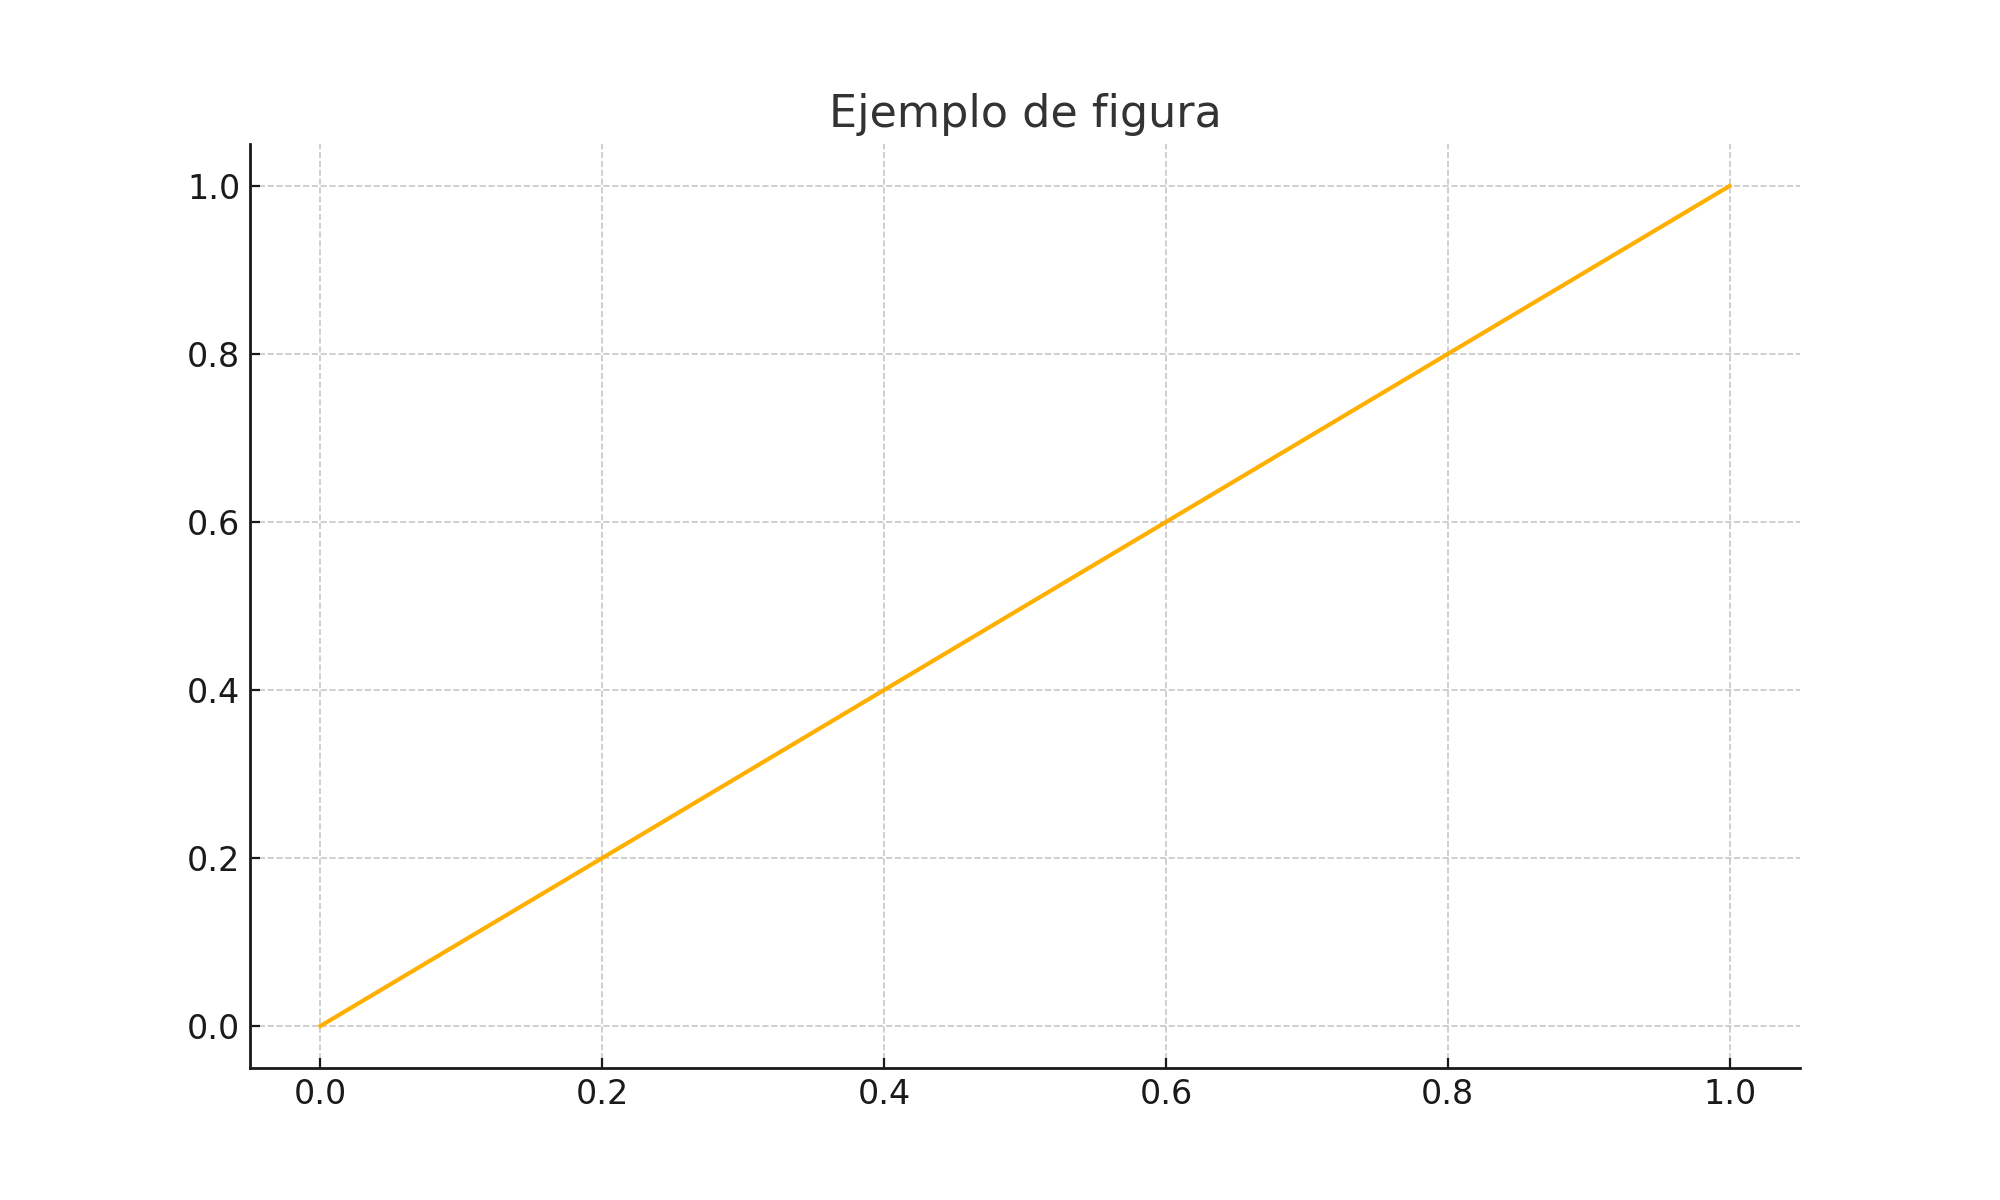
\includegraphics[width=0.7\textwidth]{assets/figura1.png}
\caption{Esquema de fuerzas y su relación. Fuente: adaptado de Hawking (2010)}
\end{figure}

\subsection*{Tablas}
\begin{table}[H]
\centering
\caption{Participación de las energías renovables primarias}
\begin{tabular}{|l|l|l|}
\hline
Región & Energías renovables & Biomasa \\
\hline
Latinoamérica & 28.9\% & 62.4\% \\
Colombia & 27.7\% & 54.4\% \\
Alemania & 3.8\% & 65.8\% \\
Mundial & 13.1\% & 79.4\% \\
\hline
\end{tabular}
\end{table}

% Diseño Metodológico
\chapterbreak
\section{Diseño Metodológico}
Describir el enfoque, fases, metodología de diagnóstico \cite{gonzalezModeloAdministracionProyectos2012} y propuesta de intervención.

% Página horizontal con tabla amplia
\clearpage
\thispagestyle{empty}
\begin{landscape}
\begin{table}[H]
\centering
\caption{Comparativo de tecnologías por país}
\begin{tabular}{|l|c|c|c|c|c|c|}
\hline
País & Solar (MW) & Eólica (MW) & Biomasa (MW) & Hidro (MW) & Geotérmica (MW) & Total Renovables (MW) \\
\hline
Colombia & 100 & 200 & 50 & 1100 & 0 & 1450 \\
Brasil & 500 & 300 & 100 & 2000 & 50 & 2950 \\
Chile & 400 & 450 & 80 & 1200 & 30 & 2160 \\
México & 600 & 700 & 120 & 1800 & 100 & 3320 \\
Perú & 250 & 300 & 60 & 1500 & 20 & 2130 \\
\hline
\end{tabular}
\end{table}
\end{landscape}

% Diagnóstico Organizacional
\chapterbreak
\section{Diagnóstico Organizacional}
\subsection*{Procesamiento estadístico de datos}
\subsection*{Análisis de resultados}

% Plan de Intervención
\chapterbreak
\section{Plan de Intervención}
Describir la propuesta de mejora/intervención a implementar.

% Conclusiones y Recomendaciones
\chapterbreak
\section{Conclusiones y Recomendaciones}
\subsection*{Conclusiones}
\subsection*{Recomendaciones}

% Referencias
\chapterbreak
\section*{Referencias}
\printbibliography[heading=bibintoc]

% Anexos
\chapterbreak
\appendix
\section*{Anexo A. Nombre del anexo}
Contenido del anexo en esta sección, puede ser reconocido de forma automática

\end{document}